\crearanexo{Movimiento lateral hacia DEV01}{anexo:movimiento_lateral_dev01}

% ---------------------------------------------------

\subsubsection*{Objetivo}

El objetivo de esta fase es identificar la estación de trabajo DEV01 dentro de la red interna y validar el acceso remoto mediante credenciales obtenidas durante fases anteriores.

\subsubsection*{Enumeración de servicios}

Una vez establecido el túnel mediante Ligolo-ng, se enumeran los servicios expuestos por DEV01:

\begin{bashbox}
sudo nmap -sV -Pn 10.10.10.20
\end{bashbox}

Resultado esperado:

\begin{configbox}
PORT     STATE SERVICE
135/tcp  open  msrpc
139/tcp  open  netbios-ssn
445/tcp  open  microsoft-ds
3389/tcp open  ms-wbt-server
\end{configbox}

La presencia del puerto \texttt{3389/tcp} indica que el servicio de Escritorio Remoto se encuentra habilitado.

\subsubsection*{Identificación del sistema}

Para obtener información adicional del equipo se pueden utilizar herramientas de enumeración SMB:

\begin{bashbox}
enum4linux-ng 10.10.10.20
\end{bashbox}

O bien:

\begin{bashbox}
netexec smb 10.10.10.20
\end{bashbox}

El equipo se identifica como una estación Windows 7 integrada en el laboratorio:

\begin{configbox}
DEV01
Windows 7 Professional
\end{configbox}

\subsubsection*{Acceso mediante RDP}

Durante la post-explotación del servidor Ubuntu se recuperaron credenciales reutilizables:

\begin{configbox}
Usuario: dev
Contraseña: dev123
\end{configbox}

Con estas credenciales se valida el acceso remoto mediante FreeRDP:

\begin{bashbox}
xfreerdp /u:dev /p:dev123 /v:10.10.10.20 /sec:rdp
\end{bashbox}

\begin{figure}[H]
    \centering
    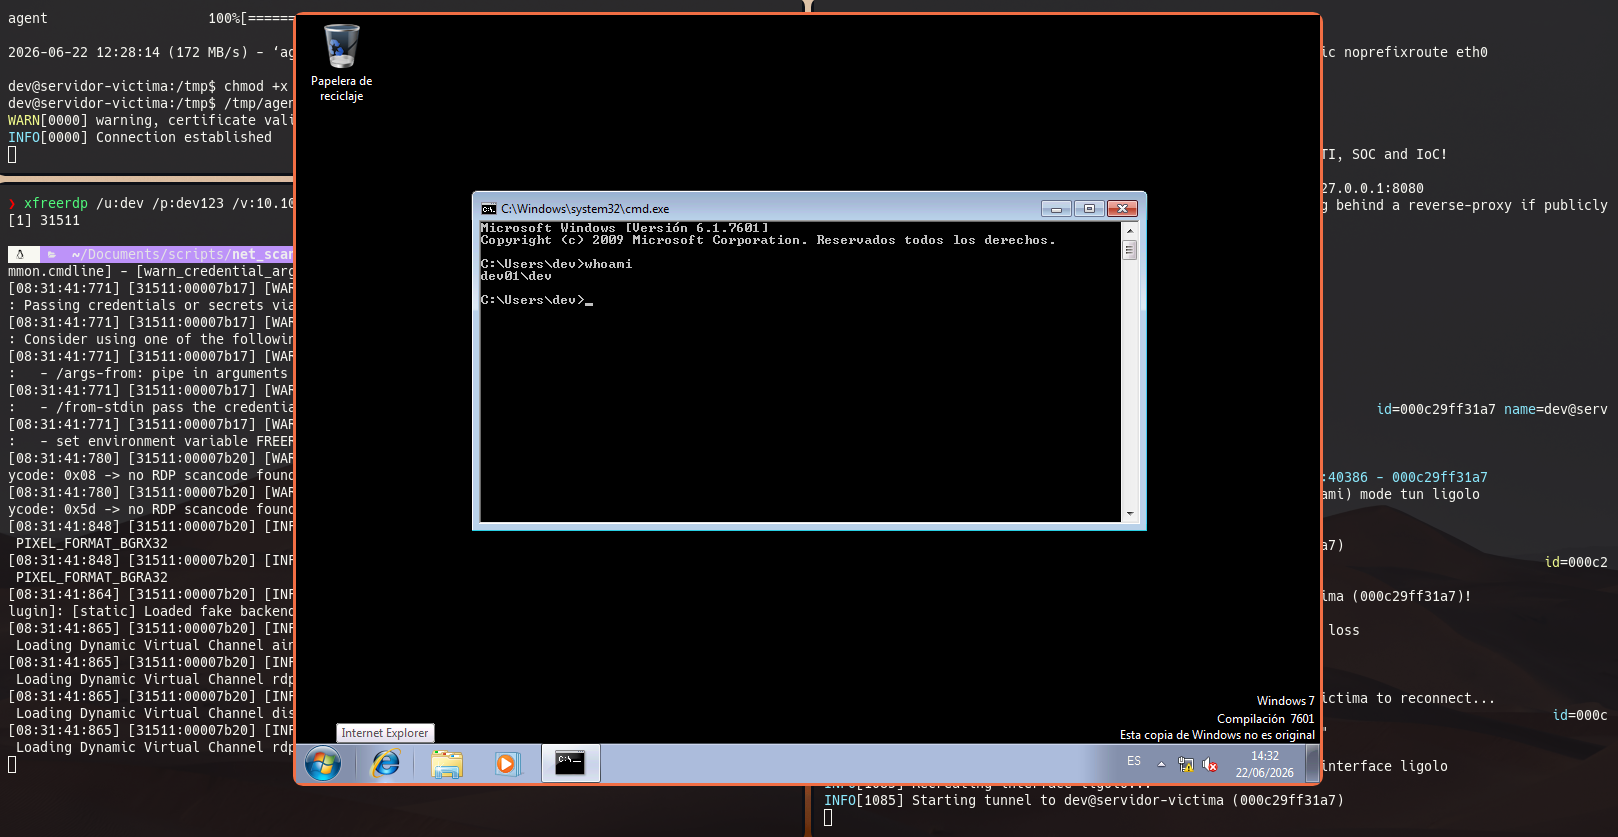
\includegraphics[width=0.95\textwidth]{Imagenes/RDP.png}

    \vspace{0.2cm}
    \captionazul{Acceso remoto a la estación DEV01 mediante RDP utilizando credenciales obtenidas previamente.}
    \label{fig:anexo_rdp_dev01}
\end{figure}

